\sect{Prüfungsaufgaben}

\ssect{FS2020}

\sssect{Aufgabe 1: Integrationsmethoden}

\begin{multicols}{2}
    a) $\int x^2 \cdot \sin(3x^3) \diff{x}$ (\textbf{Substitution})

    $u = 3x^3 \quad \quad u' = 9x^2 \quad \rightarrow \quad \diff{x} = \frac{\diff{u}}{9x^2}$
    \begin{align*}
        \int x^2 \cdot \sin(3x^3) \diff{x} &= \int x^2 \cdot \sin(u) \cdot \frac{\diff{u}}{9x^2} \\
        &= \int \frac{\sin(u)}{9} \diff{u} \\
        &= - \frac{\cos(u)}{9} + C \\
        &= - \frac{1}{9} \cos(3x^3) + C
    \end{align*}

    \columnbreak

    b) $\int \limits_{0}^{1} 5x \cdot e^{2x} \diff{x}$ (\textbf{Partielle Integration})

    $u = 5x \quad\quad u' = 5 \quad\quad v' = e^{2x} \quad\quad v = \frac{1}{2} e^{2x}$
    \begin{align*}
        \int \limits_{0}^{1} 5x \cdot e^{2x} \diff{x} &= \left[ \frac{5}{2} x \cdot e^{2x} \right]_{0}^{1} - \int \limits_{0}^{1} \frac{5}{2} e^{2x} \diff{x} \\
        &= \frac{5}{2} e^2 - \left[ \frac{5}{4} e^{2x} \right]_{0}^{1} \\
        &= \frac{5}{2} e^2 - (\frac{5}{4} e^2 - \frac{5}{4}) \\
        &= \frac{5}{4} e^2 + \frac{5}{4} = \frac{5}{4} (e^2 + 1)
    \end{align*}
\end{multicols}

c) $\int \frac{2x}{(x + 1)(x - 3)} \diff{x}$ (\textbf{Partialbruchzerlegung})

Ansatz: $\frac{2x}{(x + 1)(x - 3)} = \frac{A}{(x + 1)} + \frac{B}{(x - 3)} \Rightarrow 2x = \frac{A\cancel{(x+1)}(x-3)}{\cancel{(x+1)}} + \frac{B(x+1)\cancel{(x-3)}}{\cancel{(x-3)}} = A(x-3) + B(x+1)$

Einsetzen: $x = 3 \Rightarrow 6 = 4B \Rightarrow B = 1.5$ und $x = -1 \Rightarrow -2 = -4A \Rightarrow A = 0.5$

Somit gilt: $\frac{2x}{(x+1)(x-3)} = \frac{0.5}{(x+1)} + \frac{1.5}{(x-3)}$

$\Rightarrow \text{ Gesuchtes Integral } = \int \frac{0.5}{x + 1} \diff{x} + \int \frac{1.5}{x - 3} \diff{x} = 0.5 \ln|x + 1| + 1.5 \ln|x - 3| $

\sssect{Aufgabe 2: Anwendung der Integralrechnung}

\begin{multicols}{2}
    Durch die Rotation der Graphen $f(x) = 3e^{0.1x}$ und $g(x) = 2 \sqrt{x}$ um die $x$-Achse entsteht der Glaskörper eines Teeglases.
    Dabei stellt $f(x)$ die Aussenwand und $g(x)$ die Innenwand des Teeglases dar.

    \textbf{a) Bestimmen Sie das Volumen (Integrationsgrenzen sind im Graphen ablesbar).
    Volumen eines Rotationskörpers}

    \columnbreak

    \begin{center}
        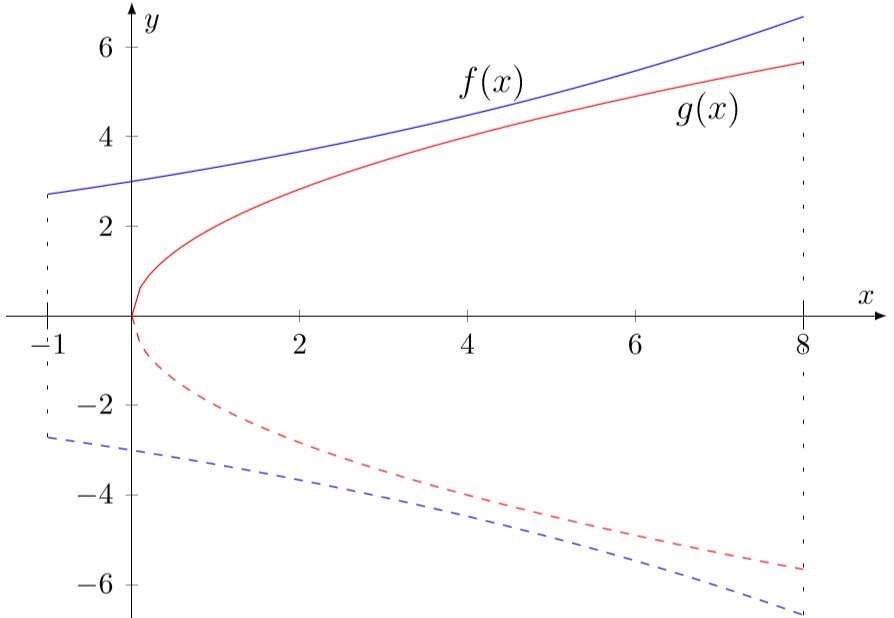
\includegraphics[scale=0.26]{fs2020-aufgabe-2}
    \end{center}
\end{multicols}

$V_1 = \pi \int \limits_{-1}^{8} f^2(x) \diff{x} = \pi \int \limits_{-1}^{8} (3e^{0.1x})^2 = \pi \int \limits_{-1}^{8} 9 e^{0.2x} = \pi \left[ 9 \cdot \frac{1}{0.2} e^{0.2x} \right]_{-1}^{8} = \pi (45 e^{1.6} - 45 e^{-0.2}) = 584.47$

$V_2 = \pi \int \limits_{0}^{8} g^2(x) \diff{x} = \pi \int \limits_{0}^{8} \left(2 \sqrt {x}\right)^2 \diff{x} = \pi \int \limits_{0}^{8} 4x \diff{x} = \pi \left[ 2x^2 \right]_0^8 = \pi \cdot 2 \cdot 64 = 128 \pi = 402.12$

$V = V_1 - V_2 = 584.47 - 402.12 = 182.35 \text{ cm}^3$

\textbf{b) Die Innenfläche (definiert durch die Rotation von $g(x)$ um die $x$-Achse) soll beschichtet werden.
Berechnen Sie die zu beschichtende Fläche.
Mantelfläche eines Rotationskörpers}

$g(x) = 2 \sqrt {x} \quad\quad g'(x) = 2 \cdot \frac{1}{2 \sqrt {x}} = \frac{1}{\sqrt {x}} \quad\quad (g'(x))^2 = \frac{1}{x}$
\begin{align*}
    \text{Gesamte Fläche: } M &= 2 \pi \cdot \int \limits_{0}^{8} y \cdot \sqrt {1 + (y')^2} \diff{x} = 2 \pi \int \limits_{0}^{8} 2 \sqrt {x} \cdot \sqrt {1 + \frac{1}{x}} \diff{x} = 2 \pi \int \limits_0^8 = 2 \sqrt {x + 1} \diff{x} = 4 \pi \int \limits_0^8 (x + 1)^\frac{1}{2} \diff{x} \\
    &= 4 \pi \left[ \frac{2}{3} (x + 1)^\frac{3}{2} \right]_0^8 = 4 \pi (\frac{2}{3} \cdot 9^\frac{3}{2} - \frac{2}{3}) = \frac{208\pi}{3} = 217.82 \text{ cm}^2
\end{align*}

\sssect{Aufgabe 3: Integrale und Grenzwerte}

\textbf{a) Berechnen Sie das Integral $\int \frac{\ln(x)}{x^2} \diff{x}$ mithilfe einer geeigneten Methode.}

\textbf{Partielle Integration:} $\quad u = \ln(x) \quad\quad u' = \frac{1}{x} \quad\quad v' = \frac{1}{x^2} = x^{-2} \quad\quad v = -x^{-1} = -\frac{1}{x}$

$\int \ln(x) \cdot \frac{1}{x^2} \diff{x} = uv - \int u'v = -\frac{\ln(x)}{x} + \int \frac{1}{x^2} \diff{x} = -\frac{\ln(x)}{x} + \int x^{-2} \diff{x} = -\frac{\ln(x)}{x} - \frac{1}{x} + C$

\textbf{b) Berechnen Sie das Integral $\int \limits_{1}^{\infty} \frac{\ln(x)}{x^2} \diff{x}$}

$\int \limits_{1}^{\infty} = \lim \limits_{t \to \infty} \int \limits_{1}^{t} \frac{\ln(x)}{x^2} = \lim \limits_{t \to \infty} \left( \left[ -\frac{\ln(x)}{x} - \frac{1}{x} \right]_{1}^{t} \right) = \lim \limits_{t \rightarrow \infty} \left( -\frac{\ln(t)}{t} - \frac{1}{t} - (0 - 1)\right) = 0 - 0 - (0 - 1) = 1$

\textbf{c) Bestimmen Sie den Grenzwert von $\lim \limits_{x \to 0} \frac{x}{\ln(3x + 1)}$}

Bernoulli-Hôpital mit $f(x) = x$ und $g(x) = \ln(3x + 1)$ anwenden:

$f'(x) = 1, g'(x) = \frac{1}{3x + 1} \cdot 3 = \frac{3}{3x + 1}$

$\frac{f'(x)}{g'(x)} = \frac{1}{\frac{3}{3x + 1}} = \frac{3x + 1}{3} \xrightarrow[x \to 0]{} \frac{1}{3}$

\textbf{d) Bestimmen Sie den Grenzwert von $\lim \limits_{x \to \infty} x \cdot \ln\left(\frac{x + 2}{x - 3}\right)$}

Umformen zu einem Bruch: \[x \cdot \ln\left( \frac{x + 2}{x - 3} \right) = \frac{\ln\left( \frac{x + 2}{x - 3} \right)}{1/x}\]

Bernoulli-Hôpital anwenden mit $f(x) = \ln \left( \frac{x + 2}{x - 3} \right)$ und $g(x) = \frac{1}{x}$:

$f'(x) = (\ln (x + 2) - \ln(x - 3))' = \frac{1}{x + 2} - \frac{1}{x - 3} = \frac{(x - 3) - (x + 2)}{(x + 2)(x - 3)} = -\frac{5}{(x + 2)(x - 3)}$

$g'(x) = (x^{-1})' = -x^{-2} = - \frac{1}{x^2}$

$\displaystyle \lim \limits_{x \to \infty} \frac{f(x)}{g(x)} = \lim \limits_{x \to \infty} \frac{f'(x)}{g'(x)} = \lim \limits_{x \to \infty} = \frac{-\frac{5}{(x + 2)(x - 3)}}{-\frac{1}{x^2}} = \lim \limits_{x \to \infty} \frac{5x^2}{(x + 2)(x - 3)} = 5$

\newpage

\sssect{Aufgabe 4: Differentialgleichungen}

Wir betrachten die Differentialgleichung \[y' \cdot y = x - 1\]

\begin{multicols}{2}
    \textbf{a) Bestimmen Sie die allgemeine Lösung.}

    $y' \cdot y = x - 1 \Rightarrow y' = \frac{x - 1}{y}$

    Separierbare DGL mit $f(x) = x - 1$ und $g(x) = \frac{1}{y}$
    \begin{align*}
        &\frac{\diff{y}}{\diff{x}} = \frac{1}{y} \cdot (x - 1) \Rightarrow \int y \cdot \diff{y} = \int (x - 1) \diff{x} \\
        &\Rightarrow \frac{y^2}{2} = \frac{x^2}{2} - x + C \Rightarrow y^2 = x^2 - 2x + 2C \\
        &\Rightarrow y = \pm \sqrt {x^2 - 2x + 2C}
    \end{align*}

    \columnbreak

    \textbf{b) Bestimmen Sie die Lösung zum Anfangswert $y(0) = 5$ und berechnen Sie den exakten Funktionswert $y(2)$}

    Da $y(0) = 5 > 0$ muss das Vorzeichen positiv sein.

    $x = 0$ und $y = 5$ einsetzen: $5 = \sqrt {0 - 0 + 2C} \Rightarrow 25 = 2C \Rightarrow C = 12.5$

    Somit: $y = \sqrt {x^2 - 2x + 25}$

    $y(2) = \sqrt {2^2 - 2 \cdot 2 + 25} = 5$
\end{multicols}

\textbf{c) Wir betrachten die obige DGL mit der Anfangsbedingung $y(0) = 5$.
Führen Sie zwei Euler-Schritte mit einer Schrittweite von $h = 1$ hintereinander durch, um den zugehörigen \emph{Schätzwert} für den Funktionswert bei $x = 2$ zu erhalten.}

$x_0 = 0, y_0 = 5, h = 1, F(x,y) = \frac{x-1}{y}$

\begin{multicols}{2}
    1. Euler-Schritt:
    \begin{align*}
        x_1 &= x_0 + h = 1 \\
        y_1 &= y_0 + h \cdot F(x_0, y_0) = 5 + 1 \cdot \frac{0 - 1}{5} = 4.8
    \end{align*}

    2. Euler-Schritt:
    \begin{align*}
        x_2 &= x_1 + h = 2 \\
        y_2 &= y_1 + h \cdot F(x_1, y_1) = 4.8 + 1 \cdot \frac{1 - 1}{4.8} = 4.8
    \end{align*}
\end{multicols}

\sssect{Aufgabe 5: Taylor-Reihen}

\textbf{a) Bestimmen Sie das Taylor-Polynom für die Funktion $f(x) = x \cdot e^x$ vom Grad $5$ um $x_0 = 0$.}

Taylor-Reihe von $e^x$ (Papula): $\displaystyle 1 + x + \frac{x^2}{2!} + \frac{x^3}{3!} + \frac{x^4}{4!} + \dots$

Taylor-Reihe von $x \cdot e^x$: $\displaystyle x \left( 1 + x + \frac{x^2}{2!} + \frac{x^3}{3!} + \frac{x^4}{4!} + \dots \right) = x + x^2 + \frac{x^3}{2!} + \frac{x^4}{3!} + \frac{x^5}{4!} + \dots$

Somit ist das gesuchte Polynom vom Grad $5$: $x + x^2 + \frac{x^3}{2} + \frac{x^4}{6} + \frac{x^5}{24}$

\textbf{b) Bestimmen Sie das Taylor-Polynom für die Funktion $g(x) = \ln(\sin(x))$ vom Grad $2$ um $x_0 = \frac{\pi}{2}$}

$\displaystyle g(x) = \ln(\sin(x)) \quad\quad g'(x) = \frac{1}{\sin(x)} \cdot \cos(x) \quad\quad g''(x) = \frac{-\sin(x) \cdot \sin(x) - \cos(x) \cdot \cos(x)}{\sin^2(x)}$

$\displaystyle g(x_0) = \ln(1) = 0 \quad\quad g'(x_0) = \frac{\cos(\pi / 2)}{\sin(\pi / 2)} = 0 \quad\quad g''(x_0) = \frac{-1}{1} = -1$

Gesuchtes Polynom:
\begin{align*}
    p_2(x) &= g(x_0) + g'(x_0) \cdot (x - x_0) + \frac{g''(x_0)}{2} \cdot (x - x_0)^2 \\
    &= 0 + 0 - \frac{1}{2} \cdot (x - \pi/2)^2 = -\frac{1}{2} (x - \pi/2)^2
\end{align*}

\textbf{c) Bestimmen Sie den Konvergenzradius der Potenzreihe $\displaystyle p(x) = \sum \limits_{k=0}^{\infty} \left( \frac{4^k}{k^2} \cdot x^k \right)$}

$\displaystyle p(x) = \sum \limits_{k=0}^{\infty} a_k \cdot (x - x_0)^k = \sum \limits_{k=0}^{\infty} \left( \frac{4^k}{k^2} \cdot x^k \right)$ mit $a_k = \frac{4^k}{k^2}$

Konvergenzradius:
$\displaystyle \lim \limits_{k \to \infty} \left| \frac{a_k}{a_{k+1}} \right| = \lim \limits_{k \to \infty} \frac{\frac{4^k}{k^2}}{\frac{4^{k+1}}{(k+1)^2}} = \lim \limits_{k \to \infty} \frac{4^k \cdot (k+1)^2}{4^{k+1} \cdot k^2} = \lim \limits_{k \to \infty} \frac{1 \cdot (k + 1)^2}{4 \cdot k^2} = \lim \limits_{k \to \infty} \frac{1}{4} \cdot \frac{(k+1)^2}{k^2} \xrightarrow[k \to \infty]{} \frac{1}{4} \cdot 1 = \frac{1}{4}$

\sssect{Aufgabe 6: Differentialgleichungen und Taylor-Reihen}

\textbf{a) Wir betrachten die DGL}
\[y' = 3 \sin(x) \cdot e^{-x^3} - 3x^2 \cdot y\]
\textbf{Bestimmen Sie die allgemeine Lösung der obigen DGL}

Umformen ergibt: $y' + \overbrace{3x^2 \cdot y}^{f(x)} = \overbrace{3 \sin(x) \cdot e^{-x^3}}^{g(x)}$

Es ist also eine lineare Differentialgleichung von der Form: $y' + f(x) \cdot y = g(x)$ mit $f(x) = 3x^2$ und $g(x) = 3\sin(x) \cdot e^{-x^3}$.

Gemäss Rezept: $F(x) = x^3$ und $y_0 = C \cdot e^{-F(x)} = C \cdot e^{-x^3}$

Somit ist $K(x) = \int g(x) \cdot e^{-F(x)} \diff{x} = \int 3 \sin(x) \cdot e^{-x^3} \cdot e^{x^3} \diff{x} = \int 3 \sin(x) \diff{x} = -3 \cos(x) + C$

Schlussendlich: $y = (-3 \cos(x) + C) \cdot e^{-x^3}$

\textbf{b) Bestimmen Sie den Konvergenzradius der Potenzreihe} $\displaystyle p(x) = \sum \limits_{k = 0}^{\infty} \frac{(2x + 1)^k}{3^k}$

Umformen ergibt:
\[\sum \limits_{k=0}^\infty \frac{(2x + 1)^k}{3^k} = \sum \limits_{k=0}^\infty \frac{(2(x + 0.5))^k}{3^k} = \sum \limits_{k=0}^\infty \frac{2^k \cdot (x + 0.5)^k}{3^k} = \sum \limits_{k=0}^\infty \frac{2^k}{3^k} \cdot (x + 0.5)^k\]

Also ist $\displaystyle a_k = \frac{2^k}{3^k} = \left( \frac{2}{3} \right)^k$

Somit ist der Konvergenzradius: $\displaystyle \lim \limits_{x \to \infty} \left| \frac{a_k}{a_{k+1}} \right| = \lim \limits_{x \to \infty} \frac{(2/3)^k}{(2/3)^{k+1}} = \lim \limits_{x \to \infty} \frac{1}{2/3} = \frac{3}{2}$